% GiveDirectly Beamer Theme (Metropolis base)
% Matching the GD presentation style from Final GD Presentation_21_11_2025.pptx

% Fonts — fontspec already loaded by Quarto/unicode-math
\setmainfont{Helvetica Neue}[
  BoldFont = Helvetica Neue Bold,
  ItalicFont = Helvetica Neue Italic
]
\setsansfont{Helvetica Neue}[
  BoldFont = Helvetica Neue Bold,
  ItalicFont = Helvetica Neue Italic
]
\setmonofont{Courier New}
\renewcommand{\familydefault}{\sfdefault}

% GiveDirectly Colors (from pptx theme)
\definecolor{GDGreen}{RGB}{21,129,88}
\definecolor{GDBlue}{RGB}{5,141,199}
\definecolor{GDBlack}{RGB}{0,0,0}
\definecolor{GDWhite}{RGB}{255,255,255}
\definecolor{GDLightGray}{RGB}{243,243,243}
\definecolor{GDDarkGray}{RGB}{51,51,51}

% Metropolis color overrides — clean white slides with green accents
\setbeamercolor{palette primary}{bg=GDGreen,fg=GDWhite}
\setbeamercolor{title separator}{fg=GDGreen}
\setbeamercolor{progress bar}{fg=GDGreen,bg=GDLightGray}
\setbeamercolor{progress bar in head/foot}{fg=GDGreen,bg=GDLightGray}
\setbeamercolor{progress bar in section page}{fg=GDGreen,bg=GDLightGray}
\setbeamercolor{frametitle}{bg=GDWhite,fg=GDBlack}
\setbeamercolor{title}{fg=GDWhite}
\setbeamercolor{subtitle}{fg=GDWhite}
\setbeamercolor{author}{fg=GDWhite}
\setbeamercolor{date}{fg=GDWhite}
\setbeamercolor{normal text}{fg=GDDarkGray,bg=GDWhite}
\setbeamercolor{alerted text}{fg=GDGreen}
\setbeamercolor{structure}{fg=GDGreen}
\setbeamercolor{block title}{fg=GDWhite,bg=GDGreen}
\setbeamercolor{block body}{fg=GDDarkGray,bg=GDLightGray}

% Metropolis settings
\metroset{
  progressbar=frametitle,
  sectionpage=progressbar,
  numbering=counter
}

% Thicker progress bar
\makeatletter
\setlength{\metropolis@progressinheadfoot@linewidth}{1.2pt}
\makeatother
\addtobeamertemplate{frametitle}{}{%
  \usebeamertemplate*{progress bar in head/foot}%
}

% Custom title page with hero image (GD style)
\usepackage{tikz}
\setbeamertemplate{title page}{
  \begin{tikzpicture}[remember picture,overlay]
    % Background image
    \node[anchor=center, inner sep=0pt] at (current page.center) {%
      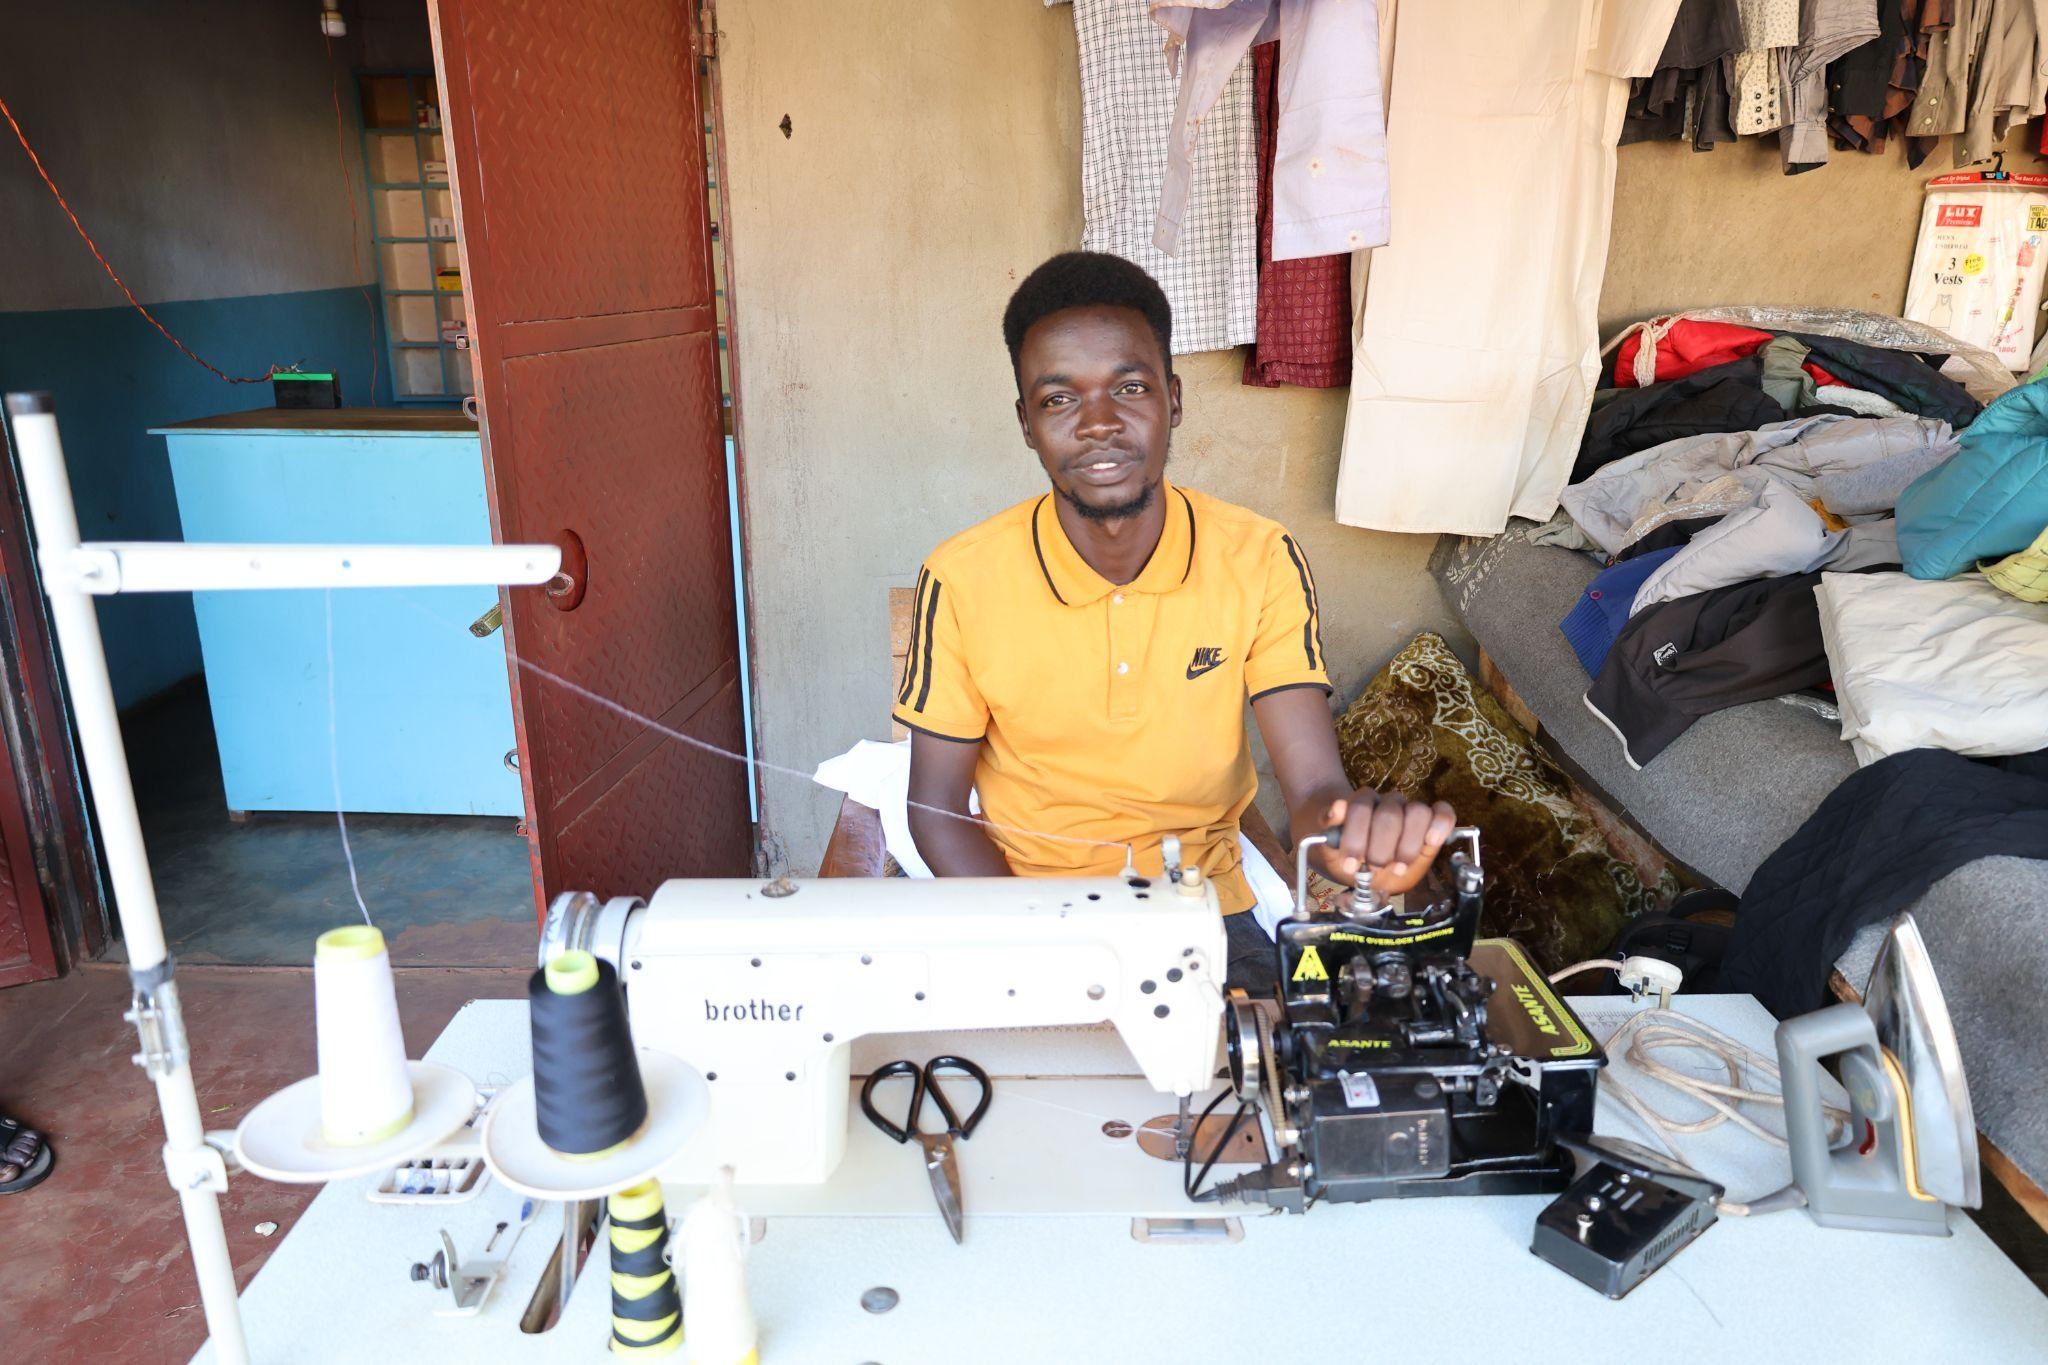
\includegraphics[width=\paperwidth,height=\paperheight,keepaspectratio=false]{figures/gd_hero.jpg}%
    };
    % Dark overlay for readability
    \fill[black,opacity=0.5] (current page.north west) rectangle (current page.south east);
    % GD Logo top-left
    \node[anchor=north west, inner sep=0pt] at ([xshift=8mm,yshift=-6mm]current page.north west) {%
      
\includegraphics[width=3.5cm]{figures/gd_logo.png}%
    };
  \end{tikzpicture}%
  \begin{minipage}[b][\paperheight]{\textwidth}
    \vfill
    \usebeamercolor[fg]{title}\usebeamerfont{title}\inserttitle\par
    \vspace*{0.5em}
    \usebeamercolor[fg]{subtitle}\usebeamerfont{subtitle}\insertsubtitle\par
    \usebeamertemplate*{title separator}
    \vspace*{1.5em}
    \usebeamercolor[fg]{author}\usebeamerfont{author}\insertauthor\par
    \vspace*{0.25em}
    \usebeamercolor[fg]{date}\usebeamerfont{date}\insertdate\par
    \vfill
    \vspace*{1mm}
  \end{minipage}
}

% Itemize styling
\setbeamertemplate{itemize items}[circle]
\setbeamertemplate{enumerate items}[default]
\usefonttheme{professionalfonts}

% Tighter spacing
\setlength{\parskip}{4pt}

% Packages
\usepackage{booktabs}
\usepackage{graphicx}
